\documentclass[svgnames]{beamer}

\usetheme{Dresden}
\usecolortheme{beaver}

\usepackage{import, fancybox, graphicx, color}

\newcommand{\ssline}{\vspace{8 pt}}

\title{Transport Protocols for Mobile Networks}

\author{Keith Winstein \\(with Anirudh Sivaraman and Hari Balakrishnan)}
\institute{M.I.T.~CSAIL}
\date{December 13, 2012}

\begin{document}

\begin{frame}[plain]

\titlepage

\end{frame}

\begin{frame}
\frametitle{The new realities}

\begin{itemize}

\item Current mobile networks differ from the traditional Internet.

\item Prior protocols perform poorly.

\item Fix the applications or fix the network?

\item Adapting applications may be easiest and best strategy.

\end{itemize}

\end{frame}

\begin{frame}
\frametitle{Outline}
\tableofcontents{}

\end{frame}

\section{Mosh: Graceful mobility}

\begin{frame}
\frametitle{Motivation: frustration with SSH}

\begin{itemize}

\item Can't roam:

\begin{itemize}
\item \ldots across Wi-Fi networks.
\item \ldots from Wi-Fi to cell or vice versa.
\end{itemize}

\item Can't sleep and wake up (usually).

\begin{itemize}
\item \ldots TCP disconnects if unacked data for too long.
\end{itemize}

\item Responds poorly to packet loss.

\item All UI requires round-trip to server.

\end{itemize}

\end{frame}

\begin{frame}

\frametitle{What we built}

\begin{enumerate}

\item Protocol for low-latency \textbf{object synchronization}

\begin{itemize}
\item with roaming
\item through suspend/resume
\item over lossy network paths
\end{itemize}

\item Supports \textbf{rolling latency compensation} on client side

\item Mobile shell application to replace SSH.

\end{enumerate}

\end{frame}

\begin{frame}

\noindent 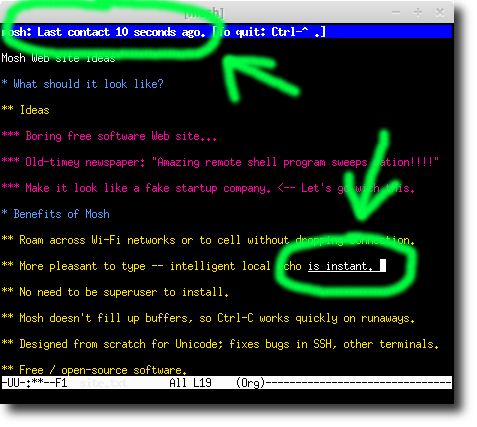
\includegraphics[scale=.5]{mosh.png}

\end{frame}

\begin{frame}
\frametitle{Demo}

\end{frame}

\begin{frame}
\frametitle{Deployment}

\begin{itemize}
\item 300,000+ page views, 75,000+ downloads, 1,500+ VCS followers.

\item Most users are on Mac OS X.

\item Included in most Linux distributions.

\item Cover of Linux Magazine.

\item Top repository of the month on GitHub.

\end{itemize}

\end{frame}

\begin{frame}
\frametitle{Twitter reviews}

\begin{itemize}
\item ``Mosh is world-changing.'' --- mftb

\item ``Mosh is the only thing that makes internet on Greyhound useful
whatsoever.'' --- standaloneSA

\item ``I'm on a train, tethering. SSH keeps failing hard. Installed
  Mosh. Instant win.'' --- maciejmalecki

\item ``Mosh gives me faith in humanity.'' --- runa

\end{itemize}

\end{frame}

\begin{frame}
\frametitle{Gmail app if user roams at the wrong time}

\textbf{July 5, 2012}:\\
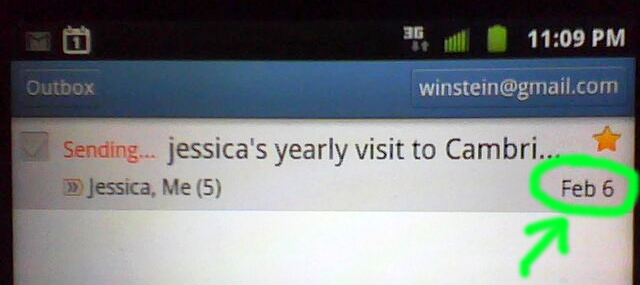
\includegraphics[scale=.5]{gmail.png}

\end{frame}

\begin{frame}
\frametitle{State synchronization for all}

Many Web and native apps have trouble with roaming and intermittent connectivity:

\begin{itemize}
\item Android Gmail app
\item Skype
\item Google Chat
\item gmail.com
\item quora.com
\item Google Voice
\item Twitter
\end{itemize}

These problems may also be expressed as state synchronization.

\end{frame}

\section{Sprout: Flow control for cellular networks}

\begin{frame}
\tableofcontents[currentsection]
\end{frame}

\begin{frame}
\frametitle{Mobile wireless networks are variable}

{\small
\def\svgwidth{\columnwidth}\input{allcapacity.pdf_tex}
}

\end{frame}

\begin{frame}
\frametitle{Mobile wireless networks are too reliable}


{\small
\def\svgwidth{2.8 in}\input{pings.pdf_tex}

Round-trip time on Verizon LTE during a TCP download.
}

\end{frame}

\begin{frame}
\frametitle{Videoconferencing systems work poorly on LTE}

\begin{itemize}
\item We measured cellular networks while driving:

\begin{itemize}
\item {\color{red}\bf Verizon LTE}
\item Verizon 3G (1xEV-DO)
\item AT\&T LTE
\item T-Mobile 3G (UMTS)
\end{itemize}

\item Then ran apps across emulated network:

\begin{itemize}
\item {\color{red}\bf Skype} (Windows 7)
\item Google Hangout (Chrome on Windows 7)
\item Apple Facetime (OS X)
\end{itemize}

\end{itemize}

\end{frame}

\begin{frame}
\frametitle{Why is performance so bad?}

\begin{itemize}
\item Exiting schemes \textbf{react} to congestion signals.

\begin{itemize}
\item Packet loss.
\item Increase in round-trip time.
\end{itemize}

\item This feedback comes too late to help.

\item The killer: \textbf{self-inflicted queueing delay}.

\item Any overshoot means a queue filling up with packets.

\end{itemize}

\end{frame}

\begin{frame}
\frametitle{Performance summary}
\vspace{-1 cm}
\def\svgwidth{\columnwidth}\footnotesize\import{dotgraphs/}{VerizonLTE-Uplink-stage0.pdf_tex}
\end{frame}

\begin{frame}
\frametitle{Sprout's goal}

\begin{itemize}
\item As much throughput as possible, with
\item bounded risk of delay $>$ 100~ms.
\end{itemize}

\end{frame}

\begin{frame}
\frametitle{Bounded risk of delay}
\begin{itemize}

\item \textbf{Infer} link speed from interarrival distribution.

\item \textbf{Predict} future link speed.

\begin{itemize}
\item Don't wait for congestion.
\end{itemize}

\item \textbf{Control:} Send as much as possible, but require:

\begin{itemize}

\item 95\% probability all packets will arrive within 100~ms.

\end{itemize}

\end{itemize}

\end{frame}

\begin{frame}
\frametitle{Infer link speed from interarrival distribution}

\def\svgwidth{0.7 \columnwidth}\input{vz-inter.pdf_tex}

\end{frame}

\begin{frame}
\frametitle{Predict future link speed}

\begin{itemize}
\item Count packets in every 20~ms tick.

\item Use Bayesian updating to infer (uncertain) link speed.

\item Make a cautious forecast.
\end{itemize}

\end{frame}

\begin{frame}

\begin{centering}
\def\svgwidth{0.85 \columnwidth}\input{sprout-model.pdf_tex}

\end{centering}

\end{frame}

%\begin{frame}
%\frametitle{The cautious forecast}
%
%\begin{itemize}
%
%\item Receiver has cloud of current link speeds
%
%\item For eight 20~ms ticks in the future:
%
%\begin{itemize}
%\item Predict future link speed
%
%\item Find 5th percentile of cumulative packets
%\end{itemize}
%
%\item Send forecast to sender (piggyback)
%
%\item Most of the math is precalculated.
%
%\end{itemize}
%\end{frame}

\begin{frame}
\frametitle{Limitations}

\begin{itemize}

\item Stochastic model has not been tuned

\item Designed for cellular link with per-user queue

\item If other users can cause you big delay, can't solve end-to-end

\end{itemize}

\end{frame}

\begin{frame}
\frametitle{Verizon LTE uplink: head-to-head}

\end{frame}

\begin{frame}
\frametitle{Verizon LTE uplink}
\vspace{-1 cm}
\def\svgwidth{\columnwidth}\footnotesize\import{dotgraphs/}{VerizonLTE-Uplink-stage0.pdf_tex}
\end{frame}

\begin{frame}
\frametitle{Verizon LTE uplink}
\vspace{-1 cm}
\def\svgwidth{\columnwidth}\footnotesize\import{dotgraphs/}{VerizonLTE-Uplink-stage1.pdf_tex}
\end{frame}

\begin{frame}
\frametitle{Verizon LTE uplink}
\vspace{-1 cm}
\def\svgwidth{\columnwidth}\footnotesize\import{dotgraphs/}{VerizonLTE-Uplink-stage2.pdf_tex}
\end{frame}

\begin{frame}
\frametitle{Verizon LTE uplink}
\vspace{-1 cm}
\def\svgwidth{\columnwidth}\footnotesize\import{dotgraphs/}{VerizonLTE-Uplink.pdf_tex}
\end{frame}

\begin{frame}
\frametitle{Verizon LTE downlink}
\vspace{-1 cm}
\def\svgwidth{\columnwidth}\footnotesize\import{dotgraphs/}{VerizonLTE-Downlink.pdf_tex}
\end{frame}

\begin{frame}
\frametitle{Verizon 3G (1xEV-DO) uplink}
\vspace{-1 cm}
\def\svgwidth{\columnwidth}\footnotesize\import{dotgraphs/}{Verizon3G1xEV-DO-Uplink.pdf_tex}
\end{frame}


\begin{frame}
\frametitle{Verizon 3G (1xEV-DO) downlink}
\vspace{-1 cm}
\def\svgwidth{\columnwidth}\footnotesize\import{dotgraphs/}{Verizon3G1xEV-DO-Downlink.pdf_tex}
\end{frame}

\begin{frame}
\frametitle{AT\&T LTE  uplink}
\vspace{-1 cm}
\def\svgwidth{\columnwidth}\footnotesize\import{dotgraphs/}{ATTLTE-Uplink.pdf_tex}
\end{frame}


\begin{frame}
\frametitle{AT\&T LTE downlink}
\vspace{-1 cm}
\def\svgwidth{\columnwidth}\footnotesize\import{dotgraphs/}{ATTLTE-Downlink.pdf_tex}
\end{frame}

\begin{frame}
\frametitle{T-Mobile 3G (UMTS)  uplink}
\vspace{-1 cm}
\def\svgwidth{\columnwidth}\footnotesize\import{dotgraphs/}{T-Mobile3GUMTS-Uplink.pdf_tex}
\end{frame}


\begin{frame}
\frametitle{T-Mobile 3G (UMTS) downlink}
\vspace{-1 cm}
\def\svgwidth{\columnwidth}\footnotesize\import{dotgraphs/}{T-Mobile3GUMTS-Downlink.pdf_tex}
\end{frame}

\begin{frame}
\frametitle{Overall results}

\begin{tabular}{|l|c|c|}
\hline
{\color{blue}Sprout} vs.~ & Avg.~speedup & Delay reduction \\
\hline
\hline
{\color{red}Skype} & $2.2\times$ & $7.9\times$ \\
{\color{red}Hangout} & $4.4\times$ & $7.2\times$ \\
{\color{red}Facetime} & $1.9\times$ & $8.7\times$ \\
\hline
{\color{ForestGreen}Compound} & $1.3\times$ & $4.8\times$ \\
{\color{ForestGreen}TCP Vegas} & $1.1\times$ & $2.1\times$ \\
{\color{ForestGreen}LEDBAT} & Same & $2.8\times$ \\
{\color{ForestGreen}Linux TCP (CUBIC)} & $1.1\times$ & $79\times$ \\
%CUBIC/CoDel & & \\
%Compound/CoDel & & \\
\hline
\end{tabular}

\end{frame}

\begin{frame}
\frametitle{Competes with AQM even though end-to-end}
\vspace{-1 cm}
\def\svgwidth{\columnwidth}\footnotesize\import{dotgraphs/}{Codels.pdf_tex}
\end{frame}

\begin{frame}
\frametitle{Future work}

\begin{itemize}
\item Public contest for best predictor
\item Anybody will be able to build protocol using results
\end{itemize}
\end{frame}

\begin{frame}
\frametitle{Sprout for controlled delay over cellular networks}

\begin{itemize}
\item \textbf{Infer} link speed from interarrival distribution

\item \textbf{Predict} future link speed

\item \textbf{Control} risk of large delay

\item Yields 2--4$\times$ throughput of Skype, Facetime, Hangout

\item Achieves 7--9$\times$ reduction in self-inflicted delay

\item Matches active queue management \textbf{without router changes}

\end{itemize}

\end{frame}

\begin{frame}
\frametitle{Conclusion}

\begin{itemize}

\item Current mobile networks differ from the traditional Internet.

\item Fix the applications or fix the network?

\item Adapting applications may be easiest and best strategy.

\item keithw@mit.edu

\end{itemize}

\end{frame}

\end{document}
